\section{Facilitate Group Assignments}

\subsection{Problem Statement}
According to the current app design, exams are answered individually. Every student has a separate answer paper and marks. A provision is required to facilitate group submissions where multiple people can simultaneously answer in the same paper. The answer sheet marks should reflect on each group member's score card.

\subsection{Design and Implementation}
Two database tables are used to store student grouping information. The first table \textbf{LabGroup} stores various group IDs for a particular Lab. The second table \textbf{StudentGroup} maps students to LabGroups, thus defining a group of students that are in a LabGroup -- writing exams as a group for a particular lab.\\

A helper function `student\_to\_group' was created which takes a student-id, course-id and lab number as arguments and returns the LabGroup ID. This was used to map students to their groups.\\

Previous design had one folder in the server per student (folder name was student id) which had his/her answers as an xml file. In-order to facilitate group assignments, one folder should be created per LabGroup (folder name should be group id to be unique). As the students answer the question paper, answers reach their group's folder. Thus simultaneous answering is possible.\\

An interface for the TAs to see the list of submissions per Lab was created, where all the LabGroups (lines showing group members) are listed as shown in figure \ref{fig:view_submissions}. Clicking on the LabGroup redirects to their answer paper. The deadline of the assignment is also shown on the top. This interface is much better than the previous ``Search for student'' interface.

\begin{figure}[H]
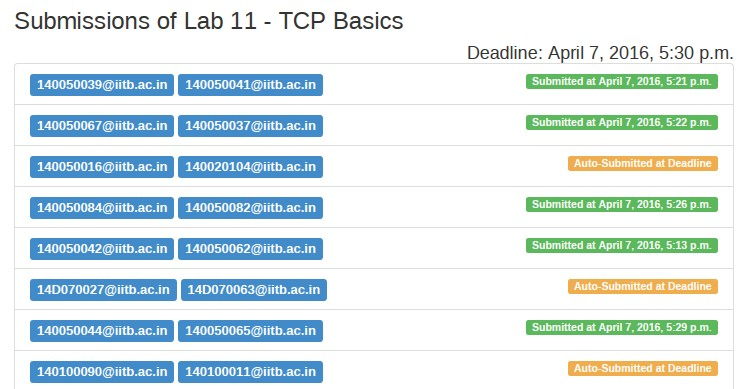
\includegraphics[width=\textwidth]{images/view_submissions}
\caption{Submissions List Page}
\label{fig:view_submissions}
\end{figure}

\subsection{Problems Faced}
Multiple (till now the maximum observed was two) LabGroups were forming for the same StudentGroups when the server load was high. On stress-testing the group-creating URL, the problem was replicated.\\

This problem was resolved in the student-to-group helper function, where if multiple LabGroups are found for a student in a particular lab, all those LabGroups (along with corresponding StudentGroups) are deleted. The students can create their group again. Unless a single Group is present for a student, the exam interface won't even be shown. This ensures that no data (answers) is lost on the above said deletion.
